
%% bare_jrnl.tex
%% V1.4b
%% 2015/08/26
%% by Michael Shell
%% see http://www.michaelshell.org/
%% for current contact information.
%%
%% This is a skeleton file demonstrating the use of IEEEtran.cls
%% (requires IEEEtran.cls version 1.8b or later) with an IEEE
%% journal paper.
%%
%% Support sites:
%% http://www.michaelshell.org/tex/ieeetran/
%% http://www.ctan.org/pkg/ieeetran
%% and
%% http://www.ieee.org/

%%*************************************************************************
%% Legal Notice:
%% This code is offered as-is without any warranty either expressed or
%% implied; without even the implied warranty of MERCHANTABILITY or
%% FITNESS FOR A PARTICULAR PURPOSE! 
%% User assumes all risk.
%% In no event shall the IEEE or any contributor to this code be liable for
%% any damages or losses, including, but not limited to, incidental,
%% consequential, or any other damages, resulting from the use or misuse
%% of any information contained here.
%%
%% All comments are the opinions of their respective authors and are not
%% necessarily endorsed by the IEEE.
%%
%% This work is distributed under the LaTeX Project Public License (LPPL)
%% ( http://www.latex-project.org/ ) version 1.3, and may be freely used,
%% distributed and modified. A copy of the LPPL, version 1.3, is included
%% in the base LaTeX documentation of all distributions of LaTeX released
%% 2003/12/01 or later.
%% Retain all contribution notices and credits.
%% ** Modified files should be clearly indicated as such, including  **
%% ** renaming them and changing author support contact information. **
%%*************************************************************************


% *** Authors should verify (and, if needed, correct) their LaTeX system  ***
% *** with the testflow diagnostic prior to trusting their LaTeX platform ***
% *** with production work. The IEEE's font choices and paper sizes can   ***
% *** trigger bugs that do not appear when using other class files.       ***                          ***
% The testflow support page is at:
% http://www.michaelshell.org/tex/testflow/



\documentclass[journal]{IEEEtran}
%
% If IEEEtran.cls has not been installed into the LaTeX system files,
% manually specify the path to it like:
% \documentclass[journal]{../sty/IEEEtran}



%---------------------------------
% Manually-included packages
\usepackage{amsmath}
\usepackage{graphicx}





% Some very useful LaTeX packages include:
% (uncomment the ones you want to load)


% *** MISC UTILITY PACKAGES ***
%
%\usepackage{ifpdf}
% Heiko Oberdiek's ifpdf.sty is very useful if you need conditional
% compilation based on whether the output is pdf or dvi.
% usage:
% \ifpdf
%   % pdf code
% \else
%   % dvi code
% \fi
% The latest version of ifpdf.sty can be obtained from:
% http://www.ctan.org/pkg/ifpdf
% Also, note that IEEEtran.cls V1.7 and later provides a builtin
% \ifCLASSINFOpdf conditional that works the same way.
% When switching from latex to pdflatex and vice-versa, the compiler may
% have to be run twice to clear warning/error messages.






% *** CITATION PACKAGES ***
%
%\usepackage{cite}
% cite.sty was written by Donald Arseneau
% V1.6 and later of IEEEtran pre-defines the format of the cite.sty package
% \cite{} output to follow that of the IEEE. Loading the cite package will
% result in citation numbers being automatically sorted and properly
% "compressed/ranged". e.g., [1], [9], [2], [7], [5], [6] without using
% cite.sty will become [1], [2], [5]--[7], [9] using cite.sty. cite.sty's
% \cite will automatically add leading space, if needed. Use cite.sty's
% noadjust option (cite.sty V3.8 and later) if you want to turn this off
% such as if a citation ever needs to be enclosed in parenthesis.
% cite.sty is already installed on most LaTeX systems. Be sure and use
% version 5.0 (2009-03-20) and later if using hyperref.sty.
% The latest version can be obtained at:
% http://www.ctan.org/pkg/cite
% The documentation is contained in the cite.sty file itself.






% *** GRAPHICS RELATED PACKAGES ***
%
\ifCLASSINFOpdf
  % \usepackage[pdftex]{graphicx}
  % declare the path(s) where your graphic files are
  % \graphicspath{{../pdf/}{../jpeg/}}
  % and their extensions so you won't have to specify these with
  % every instance of \includegraphics
  % \DeclareGraphicsExtensions{.pdf,.jpeg,.png}
\else
  % or other class option (dvipsone, dvipdf, if not using dvips). graphicx
  % will default to the driver specified in the system graphics.cfg if no
  % driver is specified.
  % \usepackage[dvips]{graphicx}
  % declare the path(s) where your graphic files are
  % \graphicspath{{../eps/}}
  % and their extensions so you won't have to specify these with
  % every instance of \includegraphics
  % \DeclareGraphicsExtensions{.eps}
\fi
% graphicx was written by David Carlisle and Sebastian Rahtz. It is
% required if you want graphics, photos, etc. graphicx.sty is already
% installed on most LaTeX systems. The latest version and documentation
% can be obtained at: 
% http://www.ctan.org/pkg/graphicx
% Another good source of documentation is "Using Imported Graphics in
% LaTeX2e" by Keith Reckdahl which can be found at:
% http://www.ctan.org/pkg/epslatex
%
% latex, and pdflatex in dvi mode, support graphics in encapsulated
% postscript (.eps) format. pdflatex in pdf mode supports graphics
% in .pdf, .jpeg, .png and .mps (metapost) formats. Users should ensure
% that all non-photo figures use a vector format (.eps, .pdf, .mps) and
% not a bitmapped formats (.jpeg, .png). The IEEE frowns on bitmapped formats
% which can result in "jaggedy"/blurry rendering of lines and letters as
% well as large increases in file sizes.
%
% You can find documentation about the pdfTeX application at:
% http://www.tug.org/applications/pdftex





% *** MATH PACKAGES ***
%
%\usepackage{amsmath}
% A popular package from the American Mathematical Society that provides
% many useful and powerful commands for dealing with mathematics.
%
% Note that the amsmath package sets \interdisplaylinepenalty to 10000
% thus preventing page breaks from occurring within multiline equations. Use:
%\interdisplaylinepenalty=2500
% after loading amsmath to restore such page breaks as IEEEtran.cls normally
% does. amsmath.sty is already installed on most LaTeX systems. The latest
% version and documentation can be obtained at:
% http://www.ctan.org/pkg/amsmath





% *** SPECIALIZED LIST PACKAGES ***
%
%\usepackage{algorithmic}
% algorithmic.sty was written by Peter Williams and Rogerio Brito.
% This package provides an algorithmic environment fo describing algorithms.
% You can use the algorithmic environment in-text or within a figure
% environment to provide for a floating algorithm. Do NOT use the algorithm
% floating environment provided by algorithm.sty (by the same authors) or
% algorithm2e.sty (by Christophe Fiorio) as the IEEE does not use dedicated
% algorithm float types and packages that provide these will not provide
% correct IEEE style captions. The latest version and documentation of
% algorithmic.sty can be obtained at:
% http://www.ctan.org/pkg/algorithms
% Also of interest may be the (relatively newer and more customizable)
% algorithmicx.sty package by Szasz Janos:
% http://www.ctan.org/pkg/algorithmicx




% *** ALIGNMENT PACKAGES ***
%
%\usepackage{array}
% Frank Mittelbach's and David Carlisle's array.sty patches and improves
% the standard LaTeX2e array and tabular environments to provide better
% appearance and additional user controls. As the default LaTeX2e table
% generation code is lacking to the point of almost being broken with
% respect to the quality of the end results, all users are strongly
% advised to use an enhanced (at the very least that provided by array.sty)
% set of table tools. array.sty is already installed on most systems. The
% latest version and documentation can be obtained at:
% http://www.ctan.org/pkg/array


% IEEEtran contains the IEEEeqnarray family of commands that can be used to
% generate multiline equations as well as matrices, tables, etc., of high
% quality.




% *** SUBFIGURE PACKAGES ***
%\ifCLASSOPTIONcompsoc
%  \usepackage[caption=false,font=normalsize,labelfont=sf,textfont=sf]{subfig}
%\else
%  \usepackage[caption=false,font=footnotesize]{subfig}
%\fi
% subfig.sty, written by Steven Douglas Cochran, is the modern replacement
% for subfigure.sty, the latter of which is no longer maintained and is
% incompatible with some LaTeX packages including fixltx2e. However,
% subfig.sty requires and automatically loads Axel Sommerfeldt's caption.sty
% which will override IEEEtran.cls' handling of captions and this will result
% in non-IEEE style figure/table captions. To prevent this problem, be sure
% and invoke subfig.sty's "caption=false" package option (available since
% subfig.sty version 1.3, 2005/06/28) as this is will preserve IEEEtran.cls
% handling of captions.
% Note that the Computer Society format requires a larger sans serif font
% than the serif footnote size font used in traditional IEEE formatting
% and thus the need to invoke different subfig.sty package options depending
% on whether compsoc mode has been enabled.
%
% The latest version and documentation of subfig.sty can be obtained at:
% http://www.ctan.org/pkg/subfig




% *** FLOAT PACKAGES ***
%
%\usepackage{fixltx2e}
% fixltx2e, the successor to the earlier fix2col.sty, was written by
% Frank Mittelbach and David Carlisle. This package corrects a few problems
% in the LaTeX2e kernel, the most notable of which is that in current
% LaTeX2e releases, the ordering of single and double column floats is not
% guaranteed to be preserved. Thus, an unpatched LaTeX2e can allow a
% single column figure to be placed prior to an earlier double column
% figure.
% Be aware that LaTeX2e kernels dated 2015 and later have fixltx2e.sty's
% corrections already built into the system in which case a warning will
% be issued if an attempt is made to load fixltx2e.sty as it is no longer
% needed.
% The latest version and documentation can be found at:
% http://www.ctan.org/pkg/fixltx2e


%\usepackage{stfloats}
% stfloats.sty was written by Sigitas Tolusis. This package gives LaTeX2e
% the ability to do double column floats at the bottom of the page as well
% as the top. (e.g., "\begin{figure*}[!b]" is not normally possible in
% LaTeX2e). It also provides a command:
%\fnbelowfloat
% to enable the placement of footnotes below bottom floats (the standard
% LaTeX2e kernel puts them above bottom floats). This is an invasive package
% which rewrites many portions of the LaTeX2e float routines. It may not work
% with other packages that modify the LaTeX2e float routines. The latest
% version and documentation can be obtained at:
% http://www.ctan.org/pkg/stfloats
% Do not use the stfloats baselinefloat ability as the IEEE does not allow
% \baselineskip to stretch. Authors submitting work to the IEEE should note
% that the IEEE rarely uses double column equations and that authors should try
% to avoid such use. Do not be tempted to use the cuted.sty or midfloat.sty
% packages (also by Sigitas Tolusis) as the IEEE does not format its papers in
% such ways.
% Do not attempt to use stfloats with fixltx2e as they are incompatible.
% Instead, use Morten Hogholm'a dblfloatfix which combines the features
% of both fixltx2e and stfloats:
%
% \usepackage{dblfloatfix}
% The latest version can be found at:
% http://www.ctan.org/pkg/dblfloatfix




%\ifCLASSOPTIONcaptionsoff
%  \usepackage[nomarkers]{endfloat}
% \let\MYoriglatexcaption\caption
% \renewcommand{\caption}[2][\relax]{\MYoriglatexcaption[#2]{#2}}
%\fi
% endfloat.sty was written by James Darrell McCauley, Jeff Goldberg and 
% Axel Sommerfeldt. This package may be useful when used in conjunction with 
% IEEEtran.cls'  captionsoff option. Some IEEE journals/societies require that
% submissions have lists of figures/tables at the end of the paper and that
% figures/tables without any captions are placed on a page by themselves at
% the end of the document. If needed, the draftcls IEEEtran class option or
% \CLASSINPUTbaselinestretch interface can be used to increase the line
% spacing as well. Be sure and use the nomarkers option of endfloat to
% prevent endfloat from "marking" where the figures would have been placed
% in the text. The two hack lines of code above are a slight modification of
% that suggested by in the endfloat docs (section 8.4.1) to ensure that
% the full captions always appear in the list of figures/tables - even if
% the user used the short optional argument of \caption[]{}.
% IEEE papers do not typically make use of \caption[]'s optional argument,
% so this should not be an issue. A similar trick can be used to disable
% captions of packages such as subfig.sty that lack options to turn off
% the subcaptions:
% For subfig.sty:
% \let\MYorigsubfloat\subfloat
% \renewcommand{\subfloat}[2][\relax]{\MYorigsubfloat[]{#2}}
% However, the above trick will not work if both optional arguments of
% the \subfloat command are used. Furthermore, there needs to be a
% description of each subfigure *somewhere* and endfloat does not add
% subfigure captions to its list of figures. Thus, the best approach is to
% avoid the use of subfigure captions (many IEEE journals avoid them anyway)
% and instead reference/explain all the subfigures within the main caption.
% The latest version of endfloat.sty and its documentation can obtained at:
% http://www.ctan.org/pkg/endfloat
%
% The IEEEtran \ifCLASSOPTIONcaptionsoff conditional can also be used
% later in the document, say, to conditionally put the References on a 
% page by themselves.




% *** PDF, URL AND HYPERLINK PACKAGES ***
%
%\usepackage{url}
% url.sty was written by Donald Arseneau. It provides better support for
% handling and breaking URLs. url.sty is already installed on most LaTeX
% systems. The latest version and documentation can be obtained at:
% http://www.ctan.org/pkg/url
% Basically, \url{my_url_here}.




% *** Do not adjust lengths that control margins, column widths, etc. ***
% *** Do not use packages that alter fonts (such as pslatex).         ***
% There should be no need to do such things with IEEEtran.cls V1.6 and later.
% (Unless specifically asked to do so by the journal or conference you plan
% to submit to, of course. )


% correct bad hyphenation here
\hyphenation{op-tical net-works semi-conduc-tor}


\begin{document}
%
% paper title
% Titles are generally capitalized except for words such as a, an, and, as,
% at, but, by, for, in, nor, of, on, or, the, to and up, which are usually
% not capitalized unless they are the first or last word of the title.
% Linebreaks \\ can be used within to get better formatting as desired.
% Do not put math or special symbols in the title.
\title{Simulataneous Robot Localization and \\Environment Mapping with \\Simulated Sensor Measurements}
%
%
% author names and IEEE memberships
% note positions of commas and nonbreaking spaces ( ~ ) LaTeX will not break
% a structure at a ~ so this keeps an author's name from being broken across
% two lines.
% use \thanks{} to gain access to the first footnote area
% a separate \thanks must be used for each paragraph as LaTeX2e's \thanks
% was not built to handle multiple paragraphs
%

\author{Swapnil~Pande
        and~Joshua~Petrin,
        ~\IEEEmembership{EECE~3892-04,~Dr.~Richard~Alan~Peters}% <-this % stops a space
%\thanks{M. Shell was with the Department
%of Electrical and Computer Engineering, Georgia Institute of Technology, Atlanta,
%GA, 30332 USA e-mail: (see http://www.michaelshell.org/contact.html).}% <-this % stops a space
%\thanks{J. Doe and J. Doe are with Anonymous University.}% <-this % stops a space
%\thanks{Manuscript received April 19, 2005; revised August 26, 2015.}
}

% note the % following the last \IEEEmembership and also \thanks - 
% these prevent an unwanted space from occurring between the last author name
% and the end of the author line. i.e., if you had this:
% 
% \author{....lastname \thanks{...} \thanks{...} }
%                     ^------------^------------^----Do not want these spaces!
%
% a space would be appended to the last name and could cause every name on that
% line to be shifted left slightly. This is one of those "LaTeX things". For
% instance, "\textbf{A} \textbf{B}" will typeset as "A B" not "AB". To get
% "AB" then you have to do: "\textbf{A}\textbf{B}"
% \thanks is no different in this regard, so shield the last } of each \thanks
% that ends a line with a % and do not let a space in before the next \thanks.
% Spaces after \IEEEmembership other than the last one are OK (and needed) as
% you are supposed to have spaces between the names. For what it is worth,
% this is a minor point as most people would not even notice if the said evil
% space somehow managed to creep in.



% The paper headers
\markboth{}%
{}
% The only time the second header will appear is for the odd numbered pages
% after the title page when using the twoside option.
% 
% *** Note that you probably will NOT want to include the author's ***
% *** name in the headers of peer review papers.                   ***
% You can use \ifCLASSOPTIONpeerreview for conditional compilation here if
% you desire.




% If you want to put a publisher's ID mark on the page you can do it like
% this:
%\IEEEpubid{0000--0000/00\$00.00~\copyright~2015 IEEE}
% Remember, if you use this you must call \IEEEpubidadjcol in the second
% column for its text to clear the IEEEpubid mark.



% use for special paper notices
%\IEEEspecialpapernotice{(Invited Paper)}




% make the title area
\maketitle

% As a general rule, do not put math, special symbols or citations
% in the abstract or keywords.
\begin{abstract}
The abstract goes here.
\end{abstract}

% Note that keywords are not normally used for peerreview papers.
%\begin{IEEEkeywords}
%IEEE, IEEEtran, journal, \LaTeX, paper, template.
%\end{IEEEkeywords}






% For peer review papers, you can put extra information on the cover
% page as needed:
% \ifCLASSOPTIONpeerreview
% \begin{center} \bfseries EDICS Category: 3-BBND \end{center}
% \fi
%
% For peerreview papers, this IEEEtran command inserts a page break and
% creates the second title. It will be ignored for other modes.
\IEEEpeerreviewmaketitle



\section{Introduction}
% The very first letter is a 2 line initial drop letter followed
% by the rest of the first word in caps.
% 
% form to use if the first word consists of a single letter:
% \IEEEPARstart{A}{demo} file is ....
% 
% form to use if you need the single drop letter followed by
% normal text (unknown if ever used by the IEEE):
% \IEEEPARstart{A}{}demo file is ....
% 
% Some journals put the first two words in caps:
% \IEEEPARstart{T}{his demo} file is ....
% 
% Here we have the typical use of a "T" for an initial drop letter
% and "HIS" in caps to complete the first word.
\IEEEPARstart{F}{or} mobile robots, self-localization is extremely important. 
A robot must know its current state to properly perform its duties and maintain its operation. 
However, localization is non-trivial due to inherent inaccuracies in actuators and sensor 
systems, as well as non-ideal environments, which introduce additional errors. Robotic mapping of unknown 
environments is equally important and poses similar problems as localization. Given that 
the robot location is known, it is difficult to build an accurate map of the environment 
due to noisy sensor measurements. 

Mapping and localization are complementary problems. Localization depends on having an 
accurate map of the environment to which to compare sensor measurements. Mapping relies 
on exactly knowing the robot location in order to accurately place features on a map. 
However, in most robotic applications, neither the precise location of a robot nor a 
map of the environment are known. 

In order to address this problem, Simulataneous Localization and Mapping (SLAM) techniques 
have been developed, which rely on probabilistic methods to build probability 
distributions of expected positions of features and the robot in a map. SLAM algorithms 
have a vast number of potential applications. For instance, they have been used to develop 
drone and land-based robotic systems capable of mapping disaster zones 
\cite{drone-response, mapping-disaster-areas}. They are being used in autonomous cars to 
safely navigate traffic. Also, they have been used to build volumetric maps of complex mines
\cite{6d-mining-slam}.

There are three main paradigms for solving the SLAM problem: The Kalman Filter, the Particle 
Filter, and Graph-based solutions. The Kalman Filter is computationally the least intensive 
of these techniques, as it parameterizes the distributions, assuming that the robot pose and landmark positions follow a Gaussian distribution. The Particle Filter utilizes Monte Carlo techniques 
to estimate the state of the robot. Graph-based solutions assume the objects around the robot 
can be approximated to a course grid landscape. \cite{prob-robots}

This project explores the Kalman Filter and its extension, the Extended Kalman Filter (EKF), 
for running a SLAM simulation. The authors believe this is best for practical application 
because most robots can implement the EKF with relative computational ease. 

The objective of this project was to apply SLAM algorithms to build autonomous capabilities 
for a robot designed to compete in the NASA Robotic Mining Competition. The robot is 
required to mine a subsurface icy-simulant (gravel) in a Martian-like environment and deposit 
it into a collector bin. The robot’s performance is scored based on the amount of simulant 
collected within a 10 minute period in addition to performance criteria such as efficiency 
mass, energy consumption, communication bandwidth usage, and dust kickup during the mining 
operation.

The competition field is a 7.38m x 3.88 m rectangle as shown in Figure \ref{fig:playing-field}. 
The robot begins the match in the start zone with an unknown position and orientation and must 
traverse the obstacle area to the mining area to collect the gravel. The gravel must be 
returned to the collector located adjacent to be counted towards the score of the match. The 
obstacle area will contain three obstacles, randomly placed in the zone. The diameter of each 
obstacle may range from 10-30 cm and the mass may range from 3-10 kg. A target or beacon may 
be placed on the collector bin as a landmark for localizing the robot. 

\begin{figure*}[!t]%{0.35\textwidth}
\centering
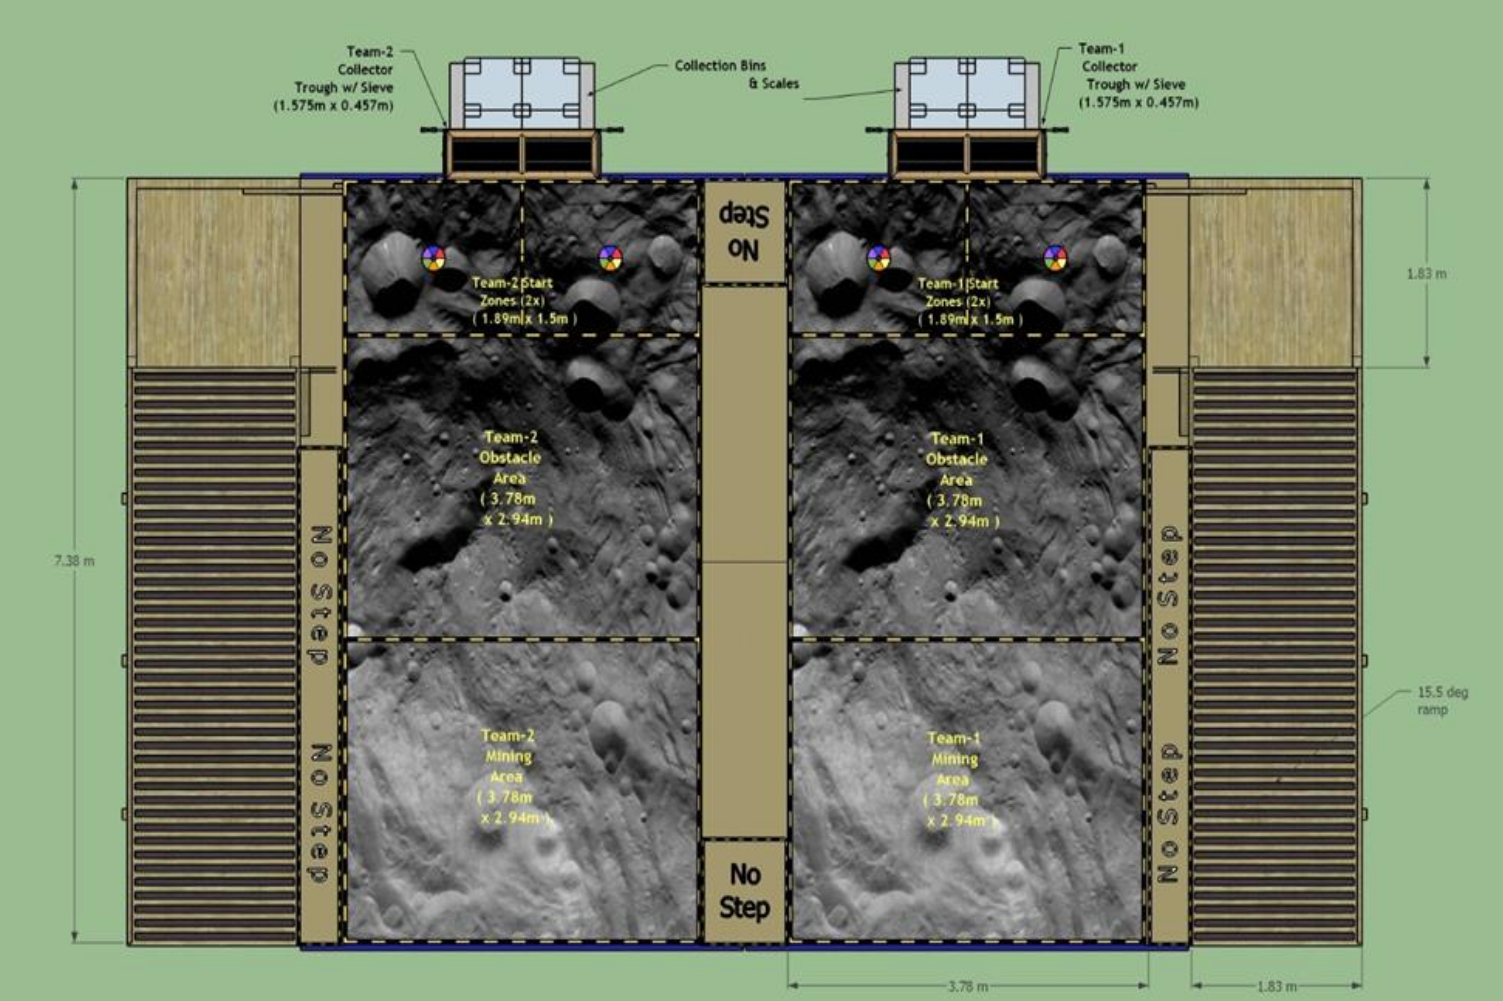
\includegraphics[width=0.9\linewidth]{Figures/playing-field.png}
\caption{Diagram of competition field \cite{nasa-rmc-rules}}
\label{fig:playing-field}
\end{figure*}

The robot is driven by 4 wheels, each with an independent drive motor and encoder. Due to 
design constraints, the robot is not capable of traversing the obstacles. The robot will be 
equipped with the following sensors:

\begin{itemize}
 \item A Microsoft Kinect to map the environment
 \item A camera with software capable of determining the location of a fiducial marker
 \item An Inertial Measurement Unit to estimate pose of the robot
\end{itemize}

The autonomy algorithm must be capable of the following tasks:

\begin{enumerate}
 \item Determining the initial pose of the robot based on data collected from the environment
 \item Traversing the obstacle zone while avoiding obstacles. 
 \item Determining when the robot has reached the mining zone and collecting gravel.
 \item Returning to the start area and depositing the gravel in the collector bin
 \item Repeating the mining process multiple times to maximize the gravel collected while 
 avoiding holes created from other mining runs.
\end{enumerate}

For the purpose of this project, the scope of the challenge was limited to localizing the robot
and determine the location of obstacles to avoid. It is assumed that a path planning algorithm 
will be capable of providing control inputs to optimize the path of the robot. This objective is 
achievable through the application of a SLAM algorithm.



\section{Methods and Procedures}

The simulation for the EKF SLAM algorithm is demonstrated through an abstract robot which 
can sense the two-dimensional environment through multiple types of sensors. The environment consisted of a fiducial marker placed at the origin and three obstacles randomly placed in the obstacle zone. To 
simulate the NASA RMC robot, the robot can sense the state of itself and the environment 
obstacles through multiple abstracted types of sensors, including:

\begin{itemize}
 \item A Microsoft Kinect, which returns a range-bearing measurment to all obstacles.
 \item A gyroscope, which can determine the robot’s angular orientation relative to its previous frame.
 \item A camera capable of determining the position of a fiducial marker placed on the collector bin.
 \item Encoders, which can determine the robot’s location relative to the previous frame. 
\end{itemize}

The Robot class (in Robot.h) represents the actual position of the robot inside its environment. 
From here, the robot can make ``measurements'' with respect to its various sensors. These 
measurements, which can be called from methods such as \texttt{getGyroMeasurement()} and 
\texttt{getArucoMeasurement()}, simply return the respective quantities the sensor is trying to 
measure, plus zero-mean gaussian noise with a preset standard deviation.  For instance, when the 
robot calls to its function \texttt{getArucoMeasurement()} while located at \texttt{(1, 1)}, the 
function may return the vector \texttt{(1.03, 0.99)} as a result of the applied sensor noise. The standard deviations were determined by collecting measurement samples from the various sensors and generating the sampling distribution.

Once these measurements are collected, the \texttt{EKFSlammer} class is instantiated. This class 
represents the robot's predicted measurements by the Extended Kalman Filter. It also represents 
the EKF's entire algorithmic complexity. The \textit{a priori} and the \textit{a posteriori} estimation steps are 
performed through several of the \texttt{EKFSlammer}'s class methods. 

\texttt{EKFSlammer} stores the robot's and environment's state $x_t$ in a \texttt{VectorXd}. The
perceived position and orientation of the robot, as well as the location of the landmarks in the map, 
can be expressed as 
\begin{equation*}
 x_t = \left[\begin{IEEEeqnarraybox*}[][c]{,c,}
        \vec{s} \\
        \theta \\
        \vec{m}_1x \\
        \vec{m}_1y \\
        \vdots
        \end{IEEEeqnarraybox*}\right],
\end{equation*}
where $\vec{s}$ is the robot's location with respect to the Aruco Marker (the arbitrarily-defined
origin) and $\vec{m}_i$ is the location of the $i$\textsuperscript{th} landmark.


First, to generate the \textit{a priori} estimate, the \texttt{motionModelUpdate()} method is called by 
\texttt{ekfUpdate}. Its parameters are the timestep for the robot and its control parameters, in 
the form of a forward velocity and an angular velocity (i.e. the \texttt{controlIn} struct; see 
\texttt{Utils.h}). The \texttt{motionModelUpdate} calculates the estimated state of the 
robot, given the control input and the known uncertainties of the robot's actuators. 

The motion model update for the \textit{a priori} estimate is defined with the following relation, given
the robot's control sequence straight-line velocity $v_t$ and angular velocity $\omega_t$:
\begin{equation*}
\left[\begin{IEEEeqnarraybox*}[][c]{,c,}
           x_{t+1} \\
           y_{t+1} \\
           \theta_{t+1}
           \end{IEEEeqnarraybox*}\right] = 
           \left[\begin{IEEEeqnarraybox*}[][c]{,c,}
           x_{t} \\
           y_{t} \\
           \theta_{t}
           \end{IEEEeqnarraybox*}\right] + 
           \left[\begin{IEEEeqnarraybox*}[][c]{,c,}
           -v_t/\omega_t \sin(\theta_t) + v_t/\omega_t \sin(\theta_t + \omega_t \Delta t)\\
           v_t/\omega_t \cos(\theta_t) - v_t/\omega_t\cos(\theta_t + \omega_t \Delta t)\\
           \omega_t \Delta t
           \end{IEEEeqnarraybox*}\right]
\end{equation*}
If covariance of the current state is $\Sigma_t$, then the Extended Kalman Filter approximates the 
covariance of the new \textit{a priori} state $\widehat{\Sigma_{t}}$ to be 
\begin{equation*}
 \widehat{\Sigma_t} = G_t \Sigma_t G_t^T + R_t,
\end{equation*}
where $G_t$ is the Jacobian of the robot's motion, and $R_t$ is a noise factor \cite{prob-robots}. Formally,
\begin{equation*}
G_t = \left[\begin{IEEEeqnarraybox*}[][c]{,c/c,}
            G^x_t & \textbf{0} \\
            \textbf{0} & I_{2N \times 2N}
           \end{IEEEeqnarraybox*}\right],
\end{equation*}
where $N$ is the number of obstacles (the quantity $2N$ above is because there are two coordinates for
each obstacle) and
\begin{equation*}
 G^x_t = \left[\begin{IEEEeqnarraybox*}[][c]{,c/c/c,}
            1\,   &  \, 0 \,  &  -v_t/\omega_t \cos(\theta_t) + v_t/\omega_t \sin(\theta_t + \omega_t \Delta t) \\
            0\,   &  \, 1 \,  &  -v_t/\omega_t \sin(\theta_t) + v_t/\omega_t \sin(\theta_t + \omega_t \Delta t) \\
            0\,   &  \, 0 \,  &   1
           \end{IEEEeqnarraybox*}\right].
\end{equation*}

Second, to generate the \textit{a posteriori} estimate, the \texttt{ekfUpdate} function calls the 
\texttt{ekfCorrectionStep}. The \texttt{ekfCorrectionStep} in turn integrates all of the sensor 
data it is passed to create a new model for the robot's and the obstacles' states. It does this 
by stepping through the Extended Kalman Filter algorithm's correction step with each set of 
sensor data. For example, \texttt{ekfCorrectionStep} will call \texttt{kinectUpdate} and pass the 
data from the Kinect sensor to correct the positions of the obstacles. 

The measurement update must calculate certain values to integrate the sensor data into the estimated
state, such as the Kalman gain $K_t$:
\begin{equation*}
 K_t = \widehat{\Sigma_t} H_t^T (H_t \widehat{\Sigma_t} H_t^T + Q_t)^{-1},
\end{equation*}
where $H_t$ is the Jacobian of each predicted sensor measurement.

The Kalman gain is a weight for the updated state and covariance to depend on the predicted state 
verses the observed state. The updated state is
\begin{equation*}
 x_{t+1} = \hat{x_t} + K_t(z_t-h(\hat{x_t})),
\end{equation*}
and the updated covariance is 
\begin{equation*}
 \Sigma_{t+1} = (I - K_t H_t) \widehat{\Sigma_t}.
\end{equation*}
This \textit{a posteriori} correction step is performed for each set of sensor data to get an accurate
value for the mean and covariance of the new state. \cite{prob-robots}


 The vectors represented
in code for measurement updates are the Kinect measurement vector and the gyroscope measurement vector.
The Kinect senses all obstacles in the environment; therefore, its measurement vector for all $i$ obstacles 
is expressed as
\begin{equation*}
 z_{t,K} = \left[\begin{IEEEeqnarraybox*}[][c]{,c,}
           r_1 \\
           \theta_1 \\
           r_2 \\
           \theta_2 \\
           \vdots \\
           r_i \\
           \theta_i
           \end{IEEEeqnarraybox*}\right] + \vec{\epsilon_t},
\end{equation*}
and the gyroscope measurement vector can be expressed as 
\begin{equation*}
 z_{t,g} = \omega_t + \epsilon_t,
\end{equation*}
where $\omega_t$ is the angular velocity of the robot, and $\vec{\epsilon_t}$ and $\epsilon_t$ are the 
normally-distributed noise factors for each sensor.

To step through a frame with a set timestep, the \texttt{ekfUpdate()} function is called. Here, the main 
method passes its control input, the perceived obstacles (from the Kinect observation), the measured 
acceleration, the measured encoder values, the measured gyroscope values, and the measured Aruco 
Marker location. \texttt{ekfUpdate} then calls all other relevant EKF functions. 



\section{Experimental Results}

The EKF SLAM algorithm was unsuccessful in accurately localizing the robot and landmarks. The 
algorithm was executed using sensor models for the Microsoft Kinect and gyro. Figures \ref{fig:1}-\ref{fig:3}
present the error between the actual and estimated pose of the robot. The estimated $x$ and $y$ positions of the 
robot did not converge to the actual positions, with errors ranging from $-1.5$ meters to $1$ meter. However, 
the estimated angular orientation of the robot closely matched the actual angular orientation with the 
difference staying within $0.2$ radians. This is likely due to the low standard deviation of the gyroscope sensor. 
Figures \ref{fig:4}-\ref{fig:6} present the variances for the estimate pose of the robot. The figures clearly demonstrate 
the effects of the prediction and correction step on the variance. The variance for each pose value 
increases during the motion model update and then decreases in the correction step with the sensor 
model updates. This accounts for the sporadic appearance of the data. However, the average variance 
reduces over time and converges to a limit. Figure \ref{fig:7} shows the number of unique landmarks stored in the 
map built by the algorithm. Despite only three landmarks being present in the environment, the algorithm 
identified 254 landmarks, indicating significant errors in data association between new observations and 
previous observations.

\begin{figure}[!t]%{0.35\textwidth}
\centering
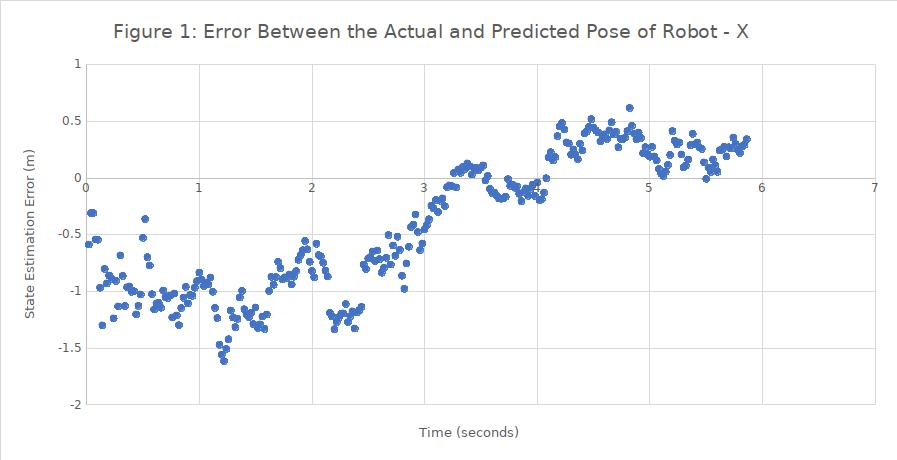
\includegraphics[width=0.9\linewidth]{Figures/1-actual-predicted-error-x.jpg}
\caption{}
\label{fig:1}
\end{figure}

\begin{figure}[!t]%{0.35\textwidth}
\centering
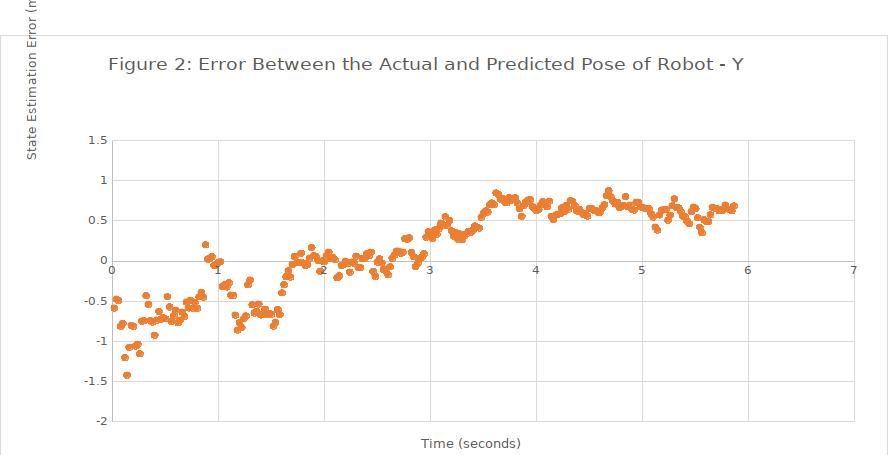
\includegraphics[width=0.9\linewidth]{Figures/2-actual-predicted-error-y.jpg}
\caption{}
\label{fig:2}
\end{figure}

\begin{figure}[!t]%{0.35\textwidth}
\centering
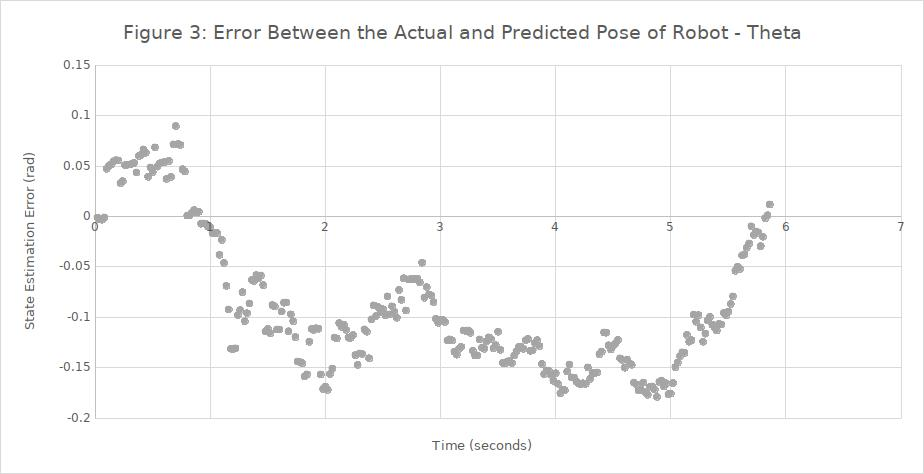
\includegraphics[width=0.9\linewidth]{Figures/3-actual-predicted-error-theta.jpg}
\caption{}
\label{fig:3}
\end{figure}

\begin{figure}[!t]%{0.35\textwidth}
\centering
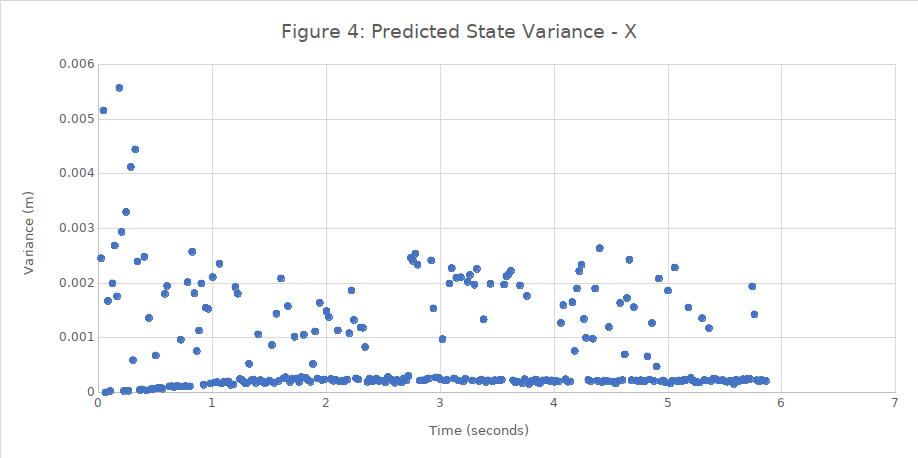
\includegraphics[width=0.9\linewidth]{Figures/4-pred-state-var-x.jpg}
\caption{}
\label{fig:4}
\end{figure}

\begin{figure}[!t]%{0.35\textwidth}
\centering
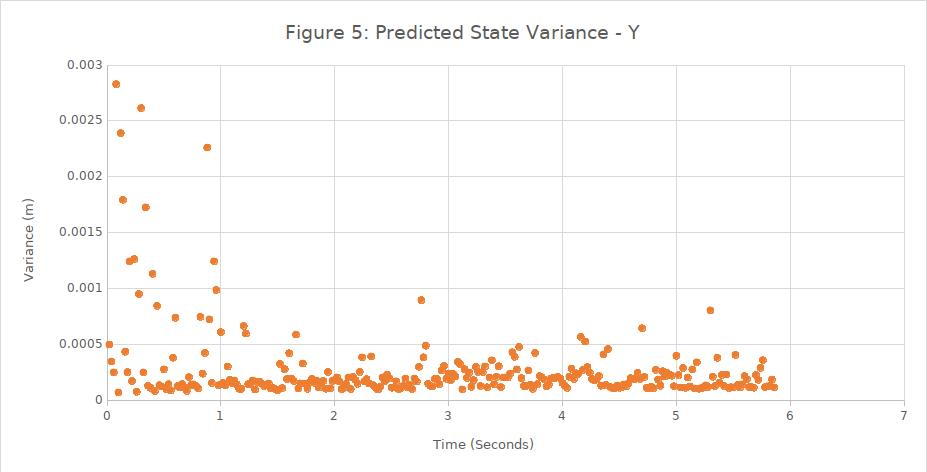
\includegraphics[width=0.9\linewidth]{Figures/5-pred-state-var-y.jpg}
\caption{}
\label{fig:5}
\end{figure}

\begin{figure}[!t]%{0.35\textwidth}
\centering
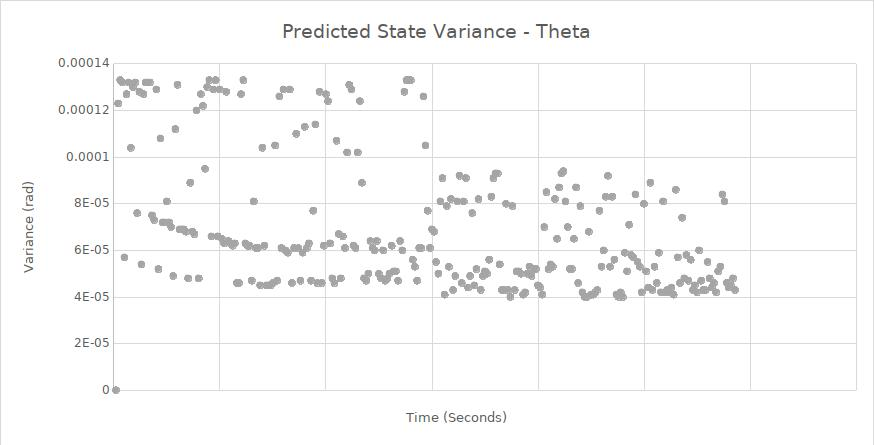
\includegraphics[width=0.9\linewidth]{Figures/6-pred-state-var-theta.jpg}
\caption{}
\label{fig:6}
\end{figure}

\begin{figure}[!t]%{0.35\textwidth}
\centering
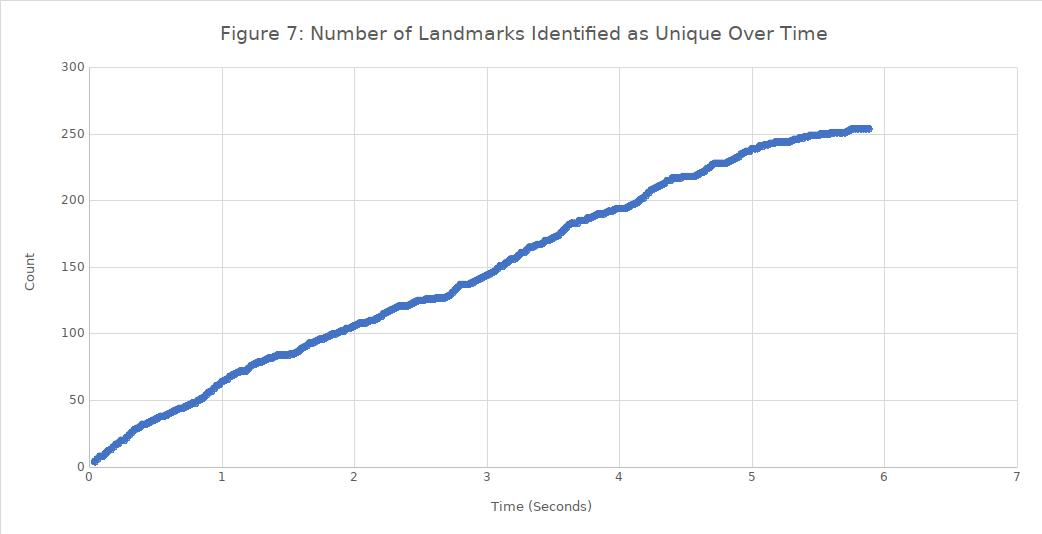
\includegraphics[width=0.9\linewidth]{Figures/7-landmarks-over-time.jpg}
\caption{}
\label{fig:7}
\end{figure}


\section{Discussion}







% An example of a floating figure using the graphicx package.
% Note that \label must occur AFTER (or within) \caption.
% For figures, \caption should occur after the \includegraphics.
% Note that IEEEtran v1.7 and later has special internal code that
% is designed to preserve the operation of \label within \caption
% even when the captionsoff option is in effect. However, because
% of issues like this, it may be the safest practice to put all your
% \label just after \caption rather than within \caption{}.
%
% Reminder: the "draftcls" or "draftclsnofoot", not "draft", class
% option should be used if it is desired that the figures are to be
% displayed while in draft mode.
%
%\begin{figure}[!t]
%\centering
%\includegraphics[width=2.5in]{myfigure}
% where an .eps filename suffix will be assumed under latex, 
% and a .pdf suffix will be assumed for pdflatex; or what has been declared
% via \DeclareGraphicsExtensions.
%\caption{Simulation results for the network.}
%\label{fig_sim}
%\end{figure}

% Note that the IEEE typically puts floats only at the top, even when this
% results in a large percentage of a column being occupied by floats.


% An example of a double column floating figure using two subfigures.
% (The subfig.sty package must be loaded for this to work.)
% The subfigure \label commands are set within each subfloat command,
% and the \label for the overall figure must come after \caption.
% \hfil is used as a separator to get equal spacing.
% Watch out that the combined width of all the subfigures on a 
% line do not exceed the text width or a line break will occur.
%
%\begin{figure*}[!t]
%\centering
%\subfloat[Case I]{\includegraphics[width=2.5in]{box}%
%\label{fig_first_case}}
%\hfil
%\subfloat[Case II]{\includegraphics[width=2.5in]{box}%
%\label{fig_second_case}}
%\caption{Simulation results for the network.}
%\label{fig_sim}
%\end{figure*}
%
% Note that often IEEE papers with subfigures do not employ subfigure
% captions (using the optional argument to \subfloat[]), but instead will
% reference/describe all of them (a), (b), etc., within the main caption.
% Be aware that for subfig.sty to generate the (a), (b), etc., subfigure
% labels, the optional argument to \subfloat must be present. If a
% subcaption is not desired, just leave its contents blank,
% e.g., \subfloat[].


% An example of a floating table. Note that, for IEEE style tables, the
% \caption command should come BEFORE the table and, given that table
% captions serve much like titles, are usually capitalized except for words
% such as a, an, and, as, at, but, by, for, in, nor, of, on, or, the, to
% and up, which are usually not capitalized unless they are the first or
% last word of the caption. Table text will default to \footnotesize as
% the IEEE normally uses this smaller font for tables.
% The \label must come after \caption as always.
%
%\begin{table}[!t]
%% increase table row spacing, adjust to taste
%\renewcommand{\arraystretch}{1.3}
% if using array.sty, it might be a good idea to tweak the value of
% \extrarowheight as needed to properly center the text within the cells
%\caption{An Example of a Table}
%\label{table_example}
%\centering
%% Some packages, such as MDW tools, offer better commands for making tables
%% than the plain LaTeX2e tabular which is used here.
%\begin{tabular}{|c||c|}
%\hline
%One & Two\\
%\hline
%Three & Four\\
%\hline
%\end{tabular}
%\end{table}


% Note that the IEEE does not put floats in the very first column
% - or typically anywhere on the first page for that matter. Also,
% in-text middle ("here") positioning is typically not used, but it
% is allowed and encouraged for Computer Society conferences (but
% not Computer Society journals). Most IEEE journals/conferences use
% top floats exclusively. 
% Note that, LaTeX2e, unlike IEEE journals/conferences, places
% footnotes above bottom floats. This can be corrected via the
% \fnbelowfloat command of the stfloats package.




\section{Conclusion}
The conclusion goes here.





% if have a single appendix:
%\appendix[Proof of the Zonklar Equations]
% or
%\appendix  % for no appendix heading
% do not use \section anymore after \appendix, only \section*
% is possibly needed

% use appendices with more than one appendix
% then use \section to start each appendix
% you must declare a \section before using any
% \subsection or using \label (\appendices by itself
% starts a section numbered zero.)
%


\appendices

% you can choose not to have a title for an appendix
% if you want by leaving the argument blank
\section{Description of Attached C++ Files}
\begin{itemize}
 \item \texttt{EKFSlammer.h} --- Defines all prediction step and correction step methods for the robot
 and obstacles, given all types of sensor inputs. 
 \item \texttt{EKFSlammer.cpp} --- Implements all the methods defined in \texttt{EKFSlammer.h}.
 \item \texttt{Robot.h} --- Defines and implements the conceptual robot and declares functions for 
  extracting (noisy) sensor measurements from the robot's defined sensors.
 \item \texttt{main.cpp} --- Creates instances of the \texttt{Robot} and the \texttt{EKFSlammer} and extracts data from
  their actual (\texttt{Robot}) results and their calculated (\texttt{EKFSlammer}) results.
 \item \texttt{Utils.h} --- Defines the \texttt{controlIn} struct, which is used to input a control to the \texttt{Robot}
  and \texttt{EKFSlammer} instances.
\end{itemize}



% use section* for acknowledgment

% Can use something like this to put references on a page
% by themselves when using endfloat and the captionsoff option.
\ifCLASSOPTIONcaptionsoff
  \newpage
\fi



% trigger a \newpage just before the given reference
% number - used to balance the columns on the last page
% adjust value as needed - may need to be readjusted if
% the document is modified later
%\IEEEtriggeratref{8}
% The "triggered" command can be changed if desired:
%\IEEEtriggercmd{\enlargethispage{-5in}}

% references section

% can use a bibliography generated by BibTeX as a .bbl file
% BibTeX documentation can be easily obtained at:
% http://mirror.ctan.org/biblio/bibtex/contrib/doc/
% The IEEEtran BibTeX style support page is at:
% http://www.michaelshell.org/tex/ieeetran/bibtex/
%\bibliographystyle{IEEEtran}
% argument is your BibTeX string definitions and bibliography database(s)
%\bibliography{IEEEabrv,../bib/paper}
%
% <OR> manually copy in the resultant .bbl file
% set second argument of \begin to the number of references
% (used to reserve space for the reference number labels box)
\begin{thebibliography}{3}

\bibitem{drone-response}
C. Alex and A. Vijaychandra, ``Autonomous cloud based drone system
for disaster response and mitigation,'' \emph{2016 International Conference 
on Robotics and Automation for Humanitarian Applications (RAHA)}, Kollam, 
2016, pp. 1-4.

\bibitem{mapping-disaster-areas}
A. Kleiner, C. Dornhege and S. Dali, ``Mapping disaster areas jointly: 
RFID-Coordinated SLAM by Hurnans and Robots,'' \emph{2007 IEEE International 
Workshop on Safety, Security and Rescue Robotics}, Rome, 2007, pp. 1-6.

\bibitem{6d-mining-slam}
A. Nuchter, H. Surmann, K. Lingemann, J. Hertzberg and S. Thrun, 
``6D SLAM with an application in autonomous mine mapping,'' 
\emph{Robotics and Automation, 2004. Proceedings. ICRA '04. 2004 IEEE 
International Conference on}, 2004, pp. 1998-2003 Vol.2.

\bibitem{prob-robots}
Sebastian Thrun, Wolfram Burgard, and Dieter Fox. 2005. \emph{Probabilistic
Robotics (Intelligent Robotics and Autonomous Agents)}. The MIT Press.

\bibitem{nasa-rmc-rules}
NASA's Ninth Annual Robotic Mining Competition Rules Rubrics, May 14-18, 
2018, Kennedy Space Center www.nasa.gov/sites/default/files/ atoms/files/%
2018\_rules\_rubrics\_parti.pdf

\end{thebibliography}

% biography section
% 
% If you have an EPS/PDF photo (graphicx package needed) extra braces are
% needed around the contents of the optional argument to biography to prevent
% the LaTeX parser from getting confused when it sees the complicated
% \includegraphics command within an optional argument. (You could create
% your own custom macro containing the \includegraphics command to make things
% simpler here.)
%\begin{IEEEbiography}[{\includegraphics[width=1in,height=1.25in,clip,keepaspectratio]{mshell}}]{Michael Shell}
% or if you just want to reserve a space for a photo:




% that's all folks
\end{document}


